\chapter{LEN5 frontend}
\section{General block diagram}
\begin{figure}[hbt]
  \centering
  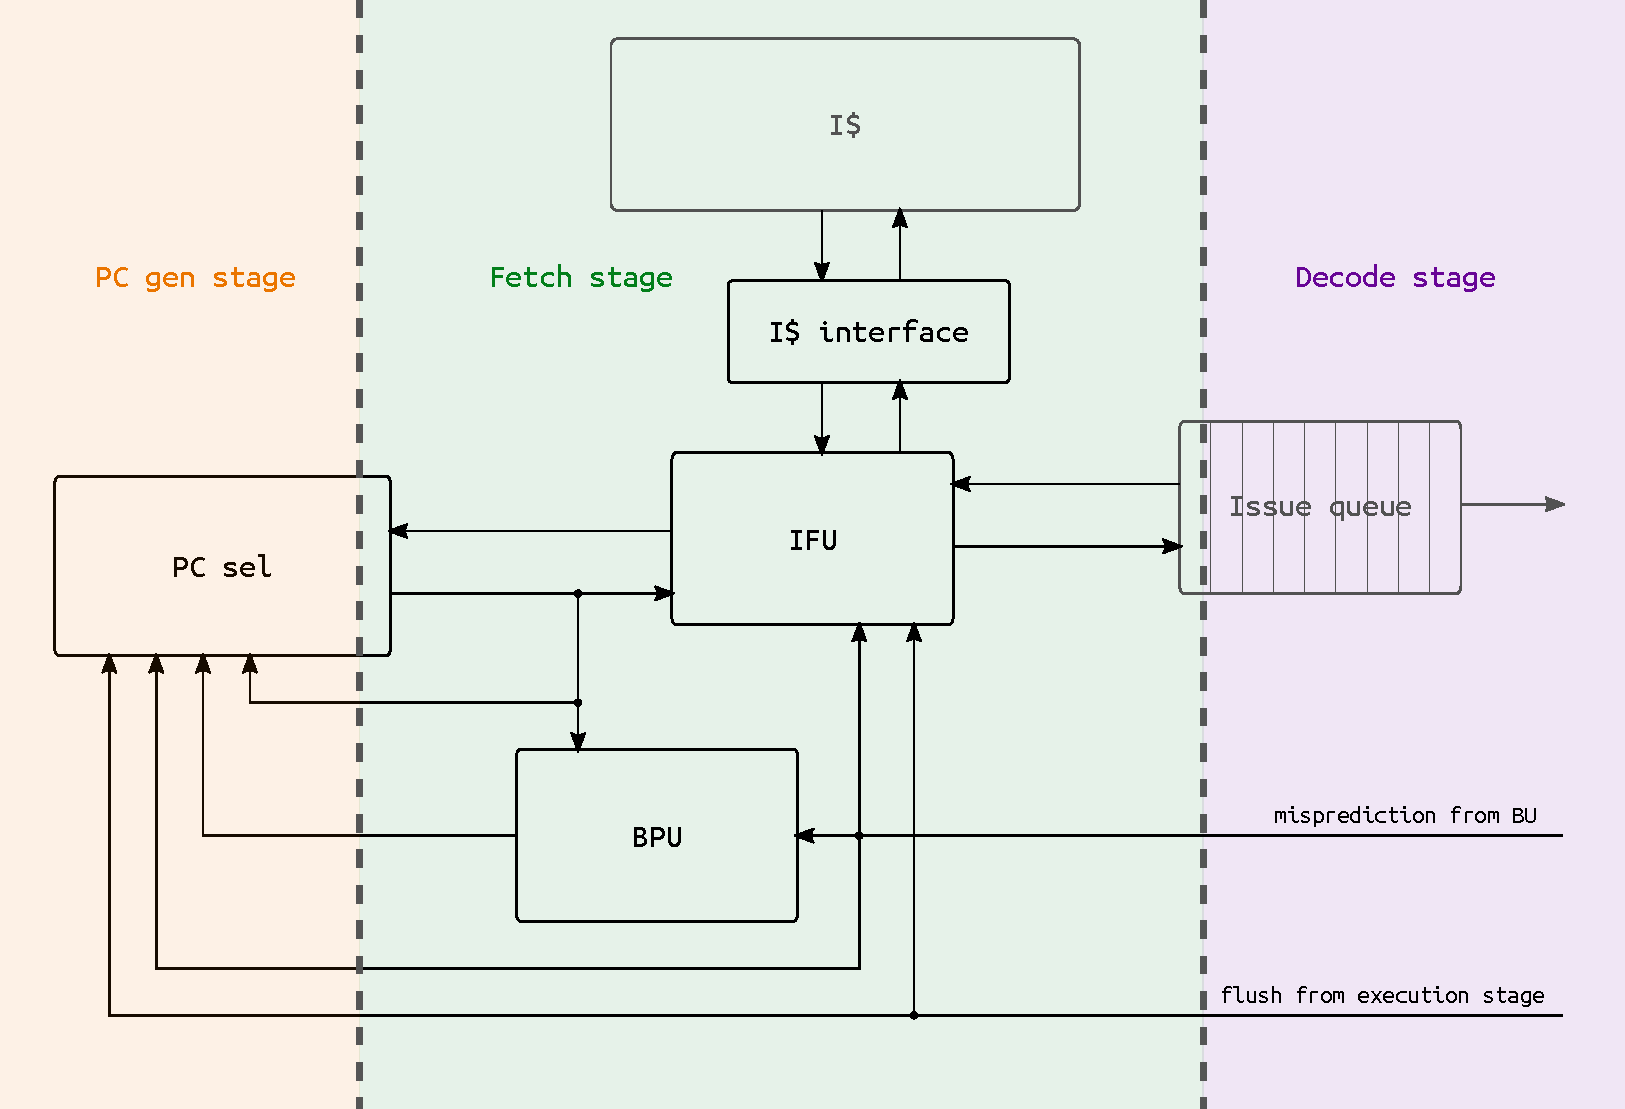
\includegraphics[width=\textwidth]{img/frontend.pdf}
  \caption{LEN5 frontend}
  \label{fig:frontend}
\end{figure}
\Cref{fig:frontend} shows a top-level block diagram of the LEN5 frontend, with the modules that were developed and that will be described in the following sections shown in solid black color. Gray blocks are instead the ones the frontend interfaces with.

The frontend is composed of two pipeline stages, name the \emph{\ac{PC} generation} and the \emph{fetch} stages. \Cref{fig:frontend} also shows the \emph{decode} stage, where the issue queue is found. This is basically a \acs{FIFO} that serves as a buffer interface between the frontend and the backend of the processor by storing a queue of instructions to be issue to the later stages of the pipeline.

In the \ac{PC} generation (\ac{PC} gen) stage the next \ac{PC} is selected among a number of different options by the \ac{PC} sel block, using a predefined priority and is then written on the output register of the stage. This register also serves as the pipeline register between the two stages, and that is why \cref{fig:frontend} shows a dashed gray line crossing the \ac{PC} sel block. The selection of the new \ac{PC} is carried out by a network of combinational logic, so that this stage always takes exactly one clock cycle.

In the fetch stage, the \ac{PC} is used by the \ac{IFU} to select and possibly read from memory the next instruction to be pushed to the issue queue. At the same time, the \ac{BPU} uses the current address to predict the next direction in case of branch and passes such information back to the \ac{PC} gen stage. Memory accesses are performed through the instruction cache interface which manages the control signals to the instruction cache. The latency of this stage is at least two clock cycles (see \cref{sec:ifu}), and in a normal steady state the \ac{IFU} can provide a throughput of one instruction each clock cycle to the issue queue, but in case of cache miss the number of cycles to resolve the stall can grow significantly, so the latency cannot be determined in advance. The issue queue is there exactly to provide some elasticity to the pipeline, by buffering already fetched instructions.

\subsection{Handshake signals}\label{sec:handshake}
The communication between each stage is always bidirectional, because in case of a stall caused for instance by a cache miss, by a full issue queue or by some other exceptional behavior down the pipeline, the \ac{PC} generation process must be interrupted along with the fetch. In order to do so, a handshake process handles the communication between each stage as well as between the instruction cache interface and the actual cache. This handshake mechanism is based on the {\smaller AXI} valid/ready protocol described below, even if it is not compliant with all the {\smaller AXI} specifications.

In each communication the source of data generates a \emph{valid} signal to indicate that the information is available, while the destination generates a \emph{ready} signal to indicate that it can accept such information \cite[p.~A3-41]{axi}. The handshake takes place and the information is successfully exchanged only at the rising clock edge when both valid and ready are asserted. For example, in \cref{fig:axi}, the handshake happens at the third rising edge of the clock.
\begin{figure}[hbt]
  \centering
  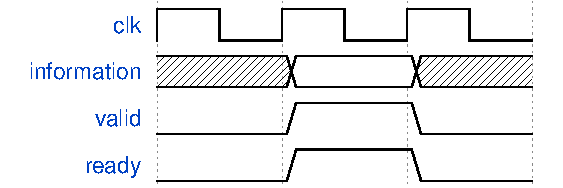
\includegraphics{img/axi.pdf}
  \caption{AXI handshake protocol}
  \label{fig:axi}
\end{figure}

When a source has information available (\cref{fig:axi_valid_ready}), it must assert valid and then wait until the corresponding ready is produced. It cannot wait for the ready before asserting valid.
\begin{figure}[hbt]
  \centering
  \subfloat[Valid before ready]{
    \label{fig:axi_valid_ready}
    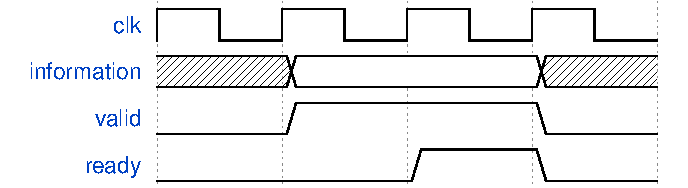
\includegraphics{img/axi_valid_ready.pdf}} \\
  \subfloat[Ready before valid]{
    \label{fig:axi_ready_valid}
    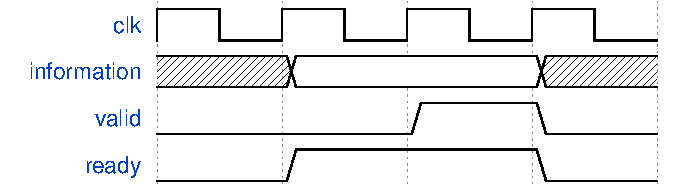
\includegraphics{img/axi_ready_valid.pdf}}
  \caption{Possible handshake timings}
  \label{fig:axi_timings}
\end{figure}
On the other hand (\cref{fig:axi_ready_valid}), a destination is allowed to wait for its valid before asserting ready and it can also deassert ready before a corresponding valid arrives.

\section{\acs{PC} gen stage}
The selection of the next \ac{PC} is based on the following list of priorities, from highest to lowest:
\begin{enumerate}
  \item \textbf{Exception}: if an exception occurs, the \ac{PC} gen stage will receive the next starting address as the base address present in the vector table provided by the {\smaller CSR} unit.
  \item \textbf{Misprediction}: if a resolved branch is discovered to have been mispredicted, then the \ac{PC} gen stage resumes execution from the correct target if the branch was actually taken, or from the next sequential address from the branch \ac{PC} if it was actually not taken.
  \item \textbf{Branch prediction}: if the \ac{BPU} predicts a taken branch for the current \ac{PC} then it provides this stage with the predicted target address (see \cref{sec:}), which will be fetched at the next cycle, thus allowing for zero penalty branches when predicted correctly.
  \item \textbf{Default assignment}: if none of the conditions before occur, then the next \ac{PC} is selected as usual as the next sequential address, which corresponds to the current \ac{PC}+4 for word-aligned 32-bit instructions.
\end{enumerate}

\begin{figure}[hbt]
  \centering
  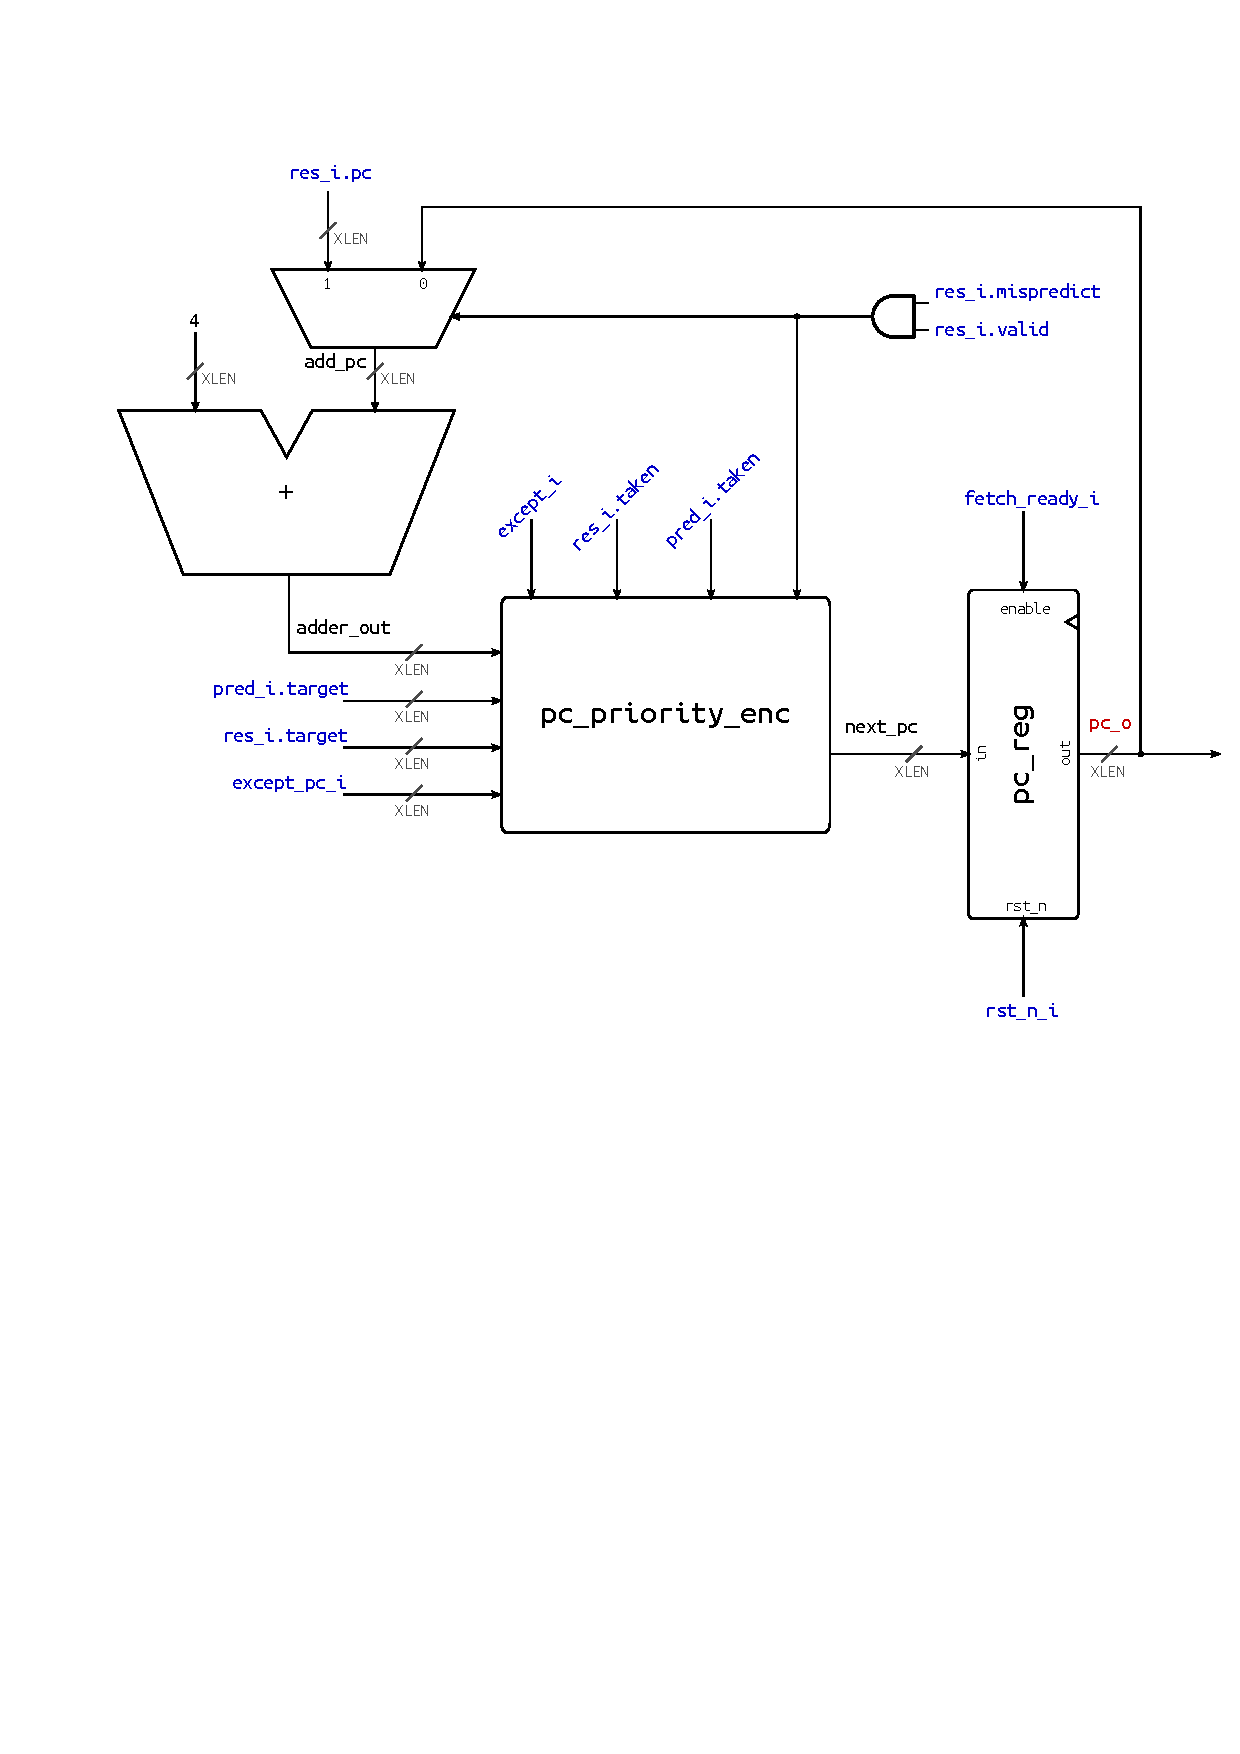
\includegraphics[width=\textwidth]{img/pc_gen_stage.pdf}
  \caption{\acs{PC} gen stage diagram}
  \label{fig:pc_gen_stage}
\end{figure}
\Cref{fig:pc_gen_stage} shows the diagram of this stage. This and all the following diagrams in this document are color coded so that input signals are in {\color{input_blue}{blue}}, output signals are in {\color{output_red}{red}}, internal signals in black and bit widths are in {\color{width_gray}{gray}}.

The heart of the \ac{PC} gen stage is the \texttt{pc\_priority\_enc} block, which is an encoder that takes as inputs all the status signals indicating a behavior different from the default and all the corresponding potential next \acp{PC}. In behavioral SystemVerilog (\cref{code:priorityenc}) it is described as a if-then-else chain, which gets synthesized as a list of cascading multiplexers implementing the desired priority\footnote{As opposed to the description using a case statement, which leads to a single parallel mux, with no priority encoded.}.
\begin{lstlisting}[
  language=Verilog,
  caption={\texttt{pc\_priority\_enc} description},
  captionpos=b,
  label=code:priorityenc
]
  always_comb begin: pc_priority_enc
    if (except_i) begin
      next_pc = except_pc_i;
    end else if (res_valid_i && res_mispredict_i) begin
      if (res_taken_i) begin
        next_pc = res_target_i;
      end else begin
        next_pc = adder_out;
      end
    end else if (pred_taken_i) begin
      next_pc = pred_target_i;
    end else begin
      next_pc = adder_out;
    end
  end: pc_priority_enc
\end{lstlisting}

In order to save resources, a single adder is used to generate both the next sequential address and the next \ac{PC} after a mispredicted not taken branch. A multiplexer driven by the misprediction signals is used to select the right operand.

The final selected next \ac{PC} is fed into the \texttt{pc\_reg} output register for the later stages. The enable of this register is controlled by the signal \texttt{fetch\_ready\_i} which comes from the fetch stage and disables the \ac{PC} generation if a stall occurs. This is part of the handshake mechanism described in \cref{sec:handshake}, even if there is no \emph{valid} signal from the \ac{PC} gen stage, as it is redundant due to the fact that a valid new \ac{PC} is always present at the output register.

\section{Instruction cache interface}
\begin{figure}[hbt]
  \centering
  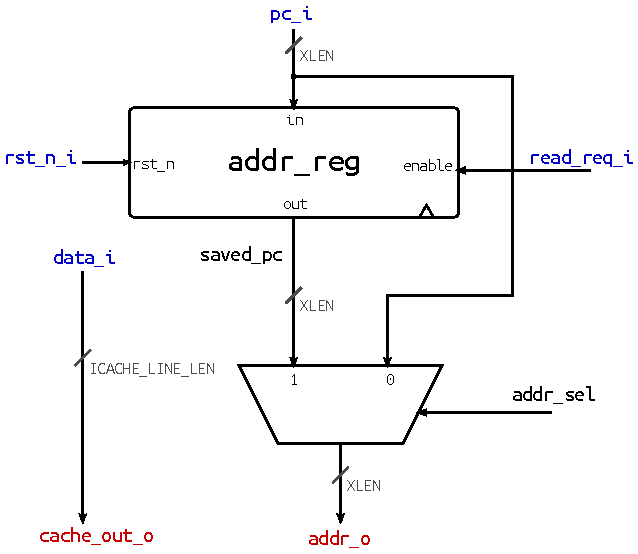
\includegraphics{img/icache_ifc.pdf}
  \caption{Instruction cache interface module ports}
  \label{fig:icache_ifc}
\end{figure}
The instruction cache interface (\cref{fig:icache_ifc}) is responsible for translating the fetch requests coming from the \ac{IFU} into compliant valid/ready handshake signals for both address and data to the instruction cache. This unit basically provides two main benefits. First, it simplifies the control of the \ac{IFU}, by delegating the handshake process. Second, and more important, it provides an additional separation layer between the core frontend and the instruction cache with modularity in mind so that, should the cache block be modified, only this interface block needs to be updated, while the signals coming from the \ac{IFU} module would remain unchanged.

\subsection{Control \acs{FSM} and timing}
While the data signals are as straightforward as simple wires connecting \texttt{pc\_i} and \texttt{cache\_out\_o} with \texttt{addr\_o} and \texttt{data\_i} respectively, the core of this interface lies in its control unit.
\begin{figure}[hbt]
  \centering
  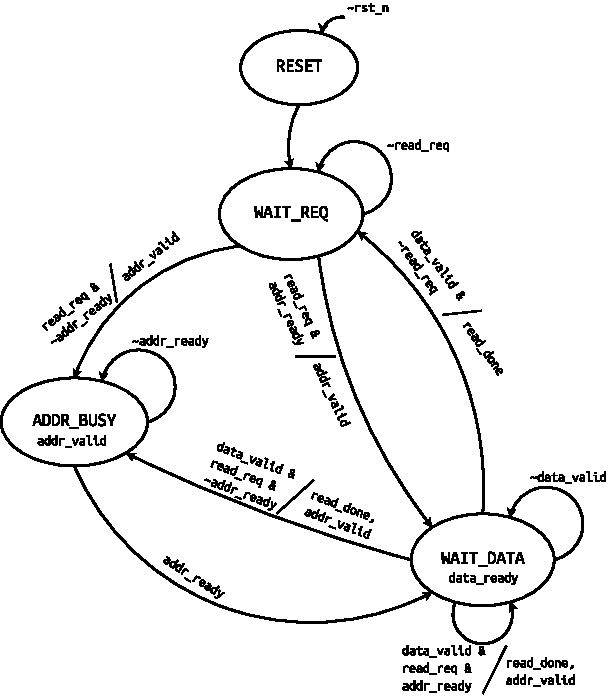
\includegraphics[scale=.8]{img/icache_ifc_fsm.pdf}
  \caption{Instruction cache interface \acs{FSM}}
  \label{fig:icache_ifc_fsm}
\end{figure}
It is a simple Mealy \acs{FSM} (\cref{fig:icache_ifc_fsm}) that after reset waits for a read request from the \ac{IFU}, then checks if the instruction cache is ready to receive an address and finally waits for a valid cache line to be read.

\begin{figure}[hbt]
  \centering
  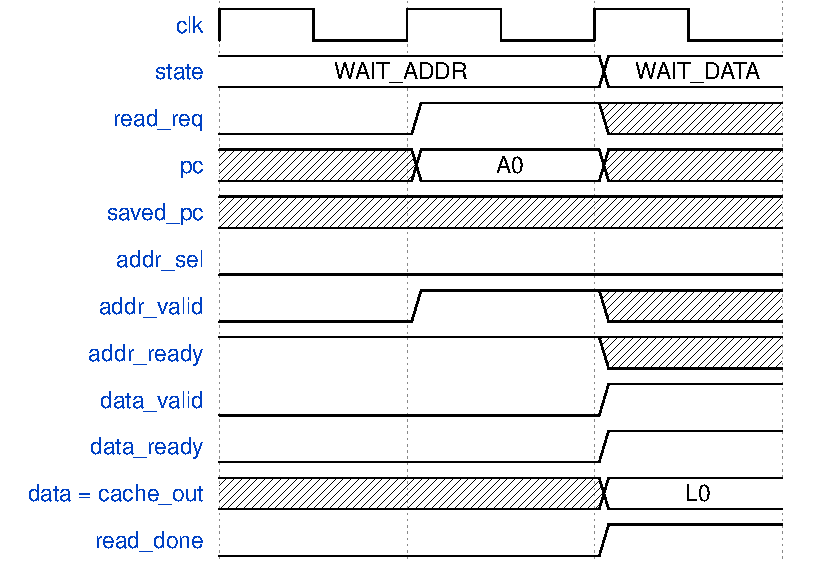
\includegraphics{img/cache01.pdf}
  \caption{Normal cache read}
  \label{fig:cache01}
\end{figure}
\Cref{fig:cache01} shows a normal cache read, where the instruction cache is immediately ready to receive an address which hits and produces the requested data at the next clock cycle. From this timing diagram it is also clear why a Mealy \acs{FSM} is needed: the signal \texttt{addr\_valid} needs to be asserted combinationally in the same clock cycle in which \texttt{read\_req} arrives, so that the address handshake can take place immediately. Otherwise, with a Moore machine, one clock cycle would be wasted at each request, rendering impossible to sustain one instruction per clock cycle fetch. Another possibility would have been not to include such signal as a Mealy output of the machine and instead connect it with a wire outside the \acs{FSM}, which would lead to the same exact result, but was deemed as less readable.

\begin{figure}[hbt]
  \centering
  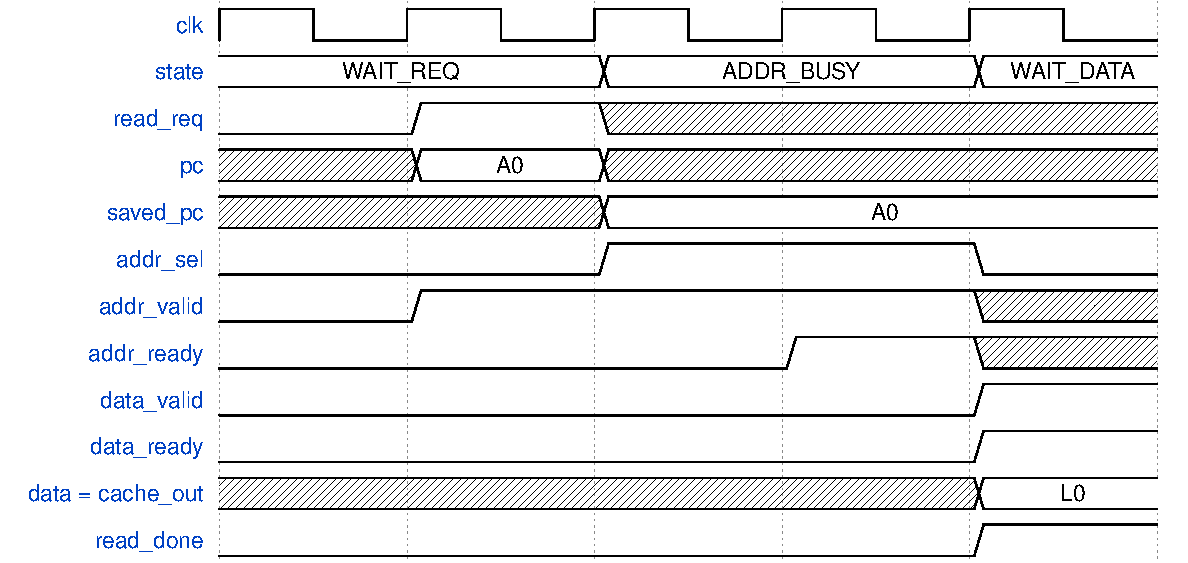
\includegraphics[width=\textwidth]{img/cache02.pdf}
  \caption{Cache not ready on address}
  \label{fig:cache02}
\end{figure}
\Cref{fig:cache02} shows another possibility when the instruction cache is not ready to receive an address at the time when a request arrives. In this case the \acs{FSM} waits until the cache become ready in the \texttt{ADDR\_BUSY} state. The state machine could just as well wait in the \texttt{WAIT\_ADDR} state, but the additional state was introduced for robustness with \texttt{addr\_valid} as a Moore output, so that this way there is no need for the \texttt{read\_req} signal to stay active until the cache is ready. This is another point in favor of a Mealy \acs{FSM} instead of the connection of combinational outputs externally.

\begin{figure}[hbt]
  \centering
  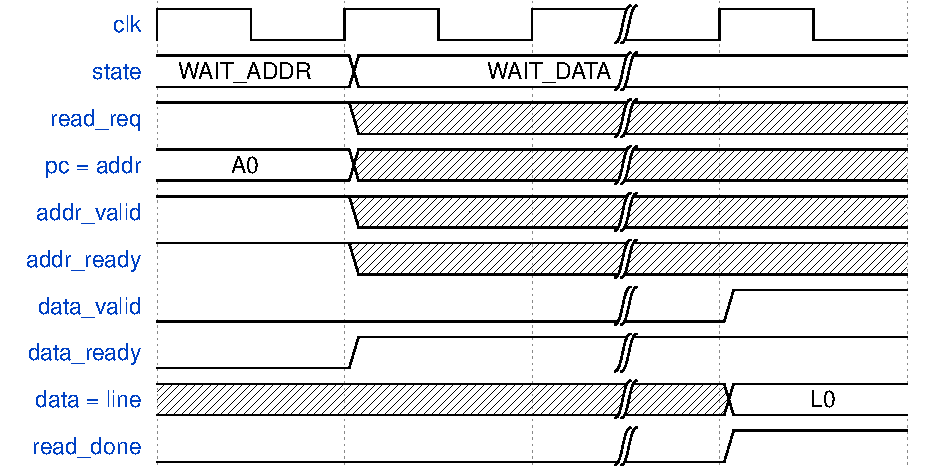
\includegraphics[width=\textwidth]{img/cache03.pdf}
  \caption{Cache miss}
  \label{fig:cache03}
\end{figure}
Finally, \cref{fig:cache03} shows the case of a cache miss, in which the \acs{FSM} waits while keeping \texttt{data\_ready} asserted. This state could potentially last for many clock cycles.

\section{\acf{IFU}}\label{sec:ifu}
\begin{figure}[hbt]
  \centering
  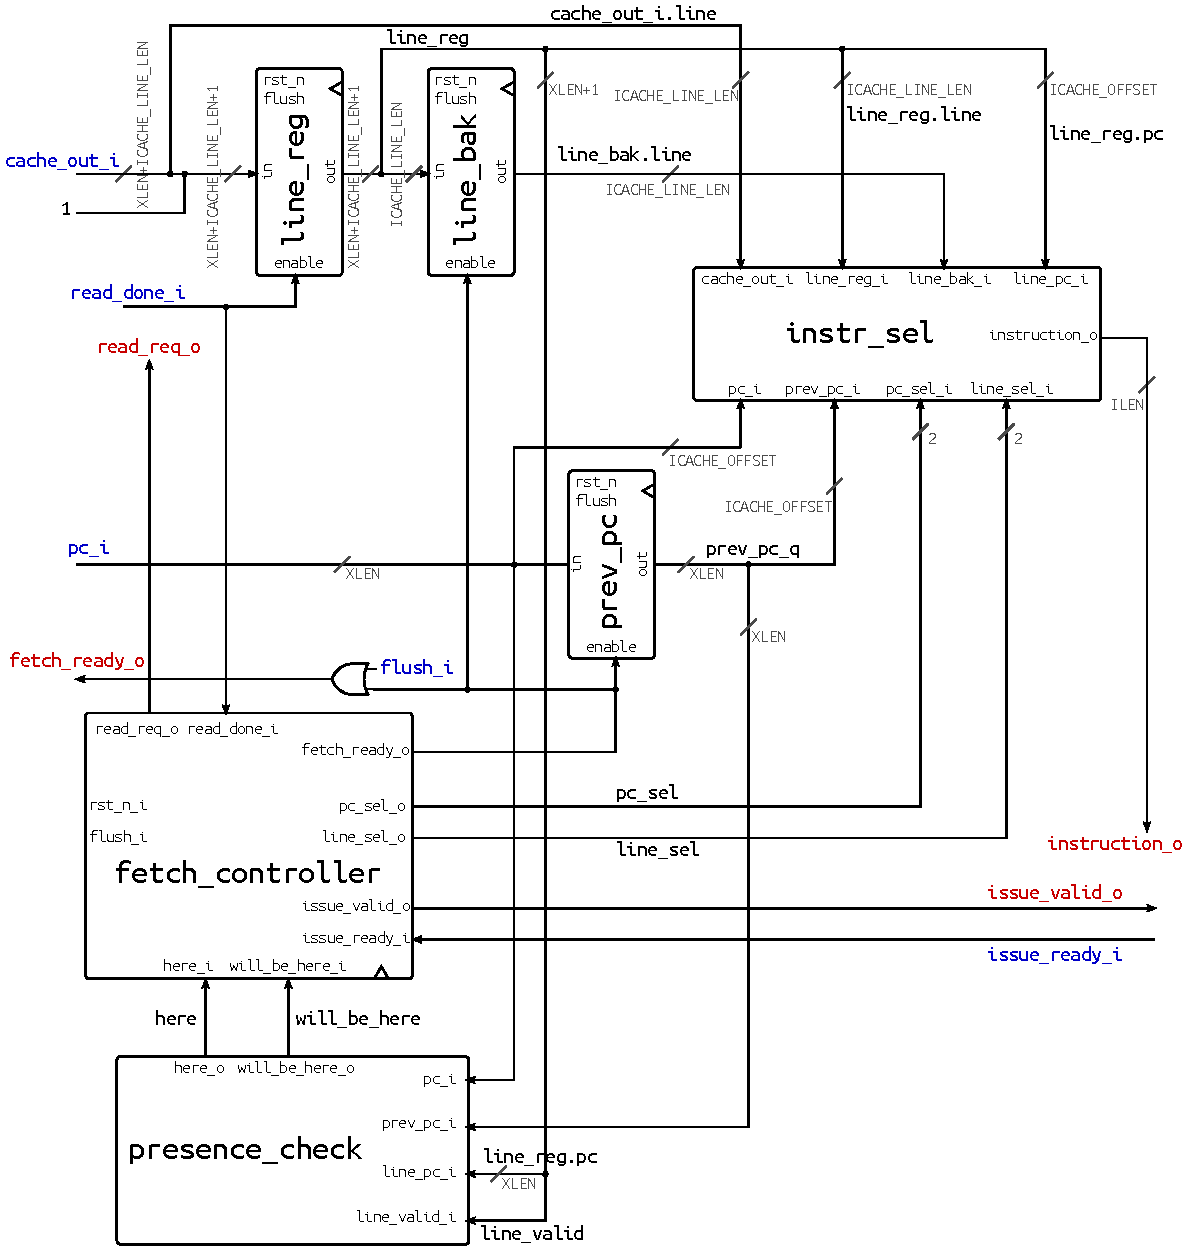
\includegraphics[width=\textwidth]{img/ifu.pdf}
  \caption[\acs{IFU} diagram]{\acs{IFU} diagram (inputs \texttt{rst\_n\_i} and \texttt{flush\_i} are shown as module port but are not connected with wires to avoid further clutter in the diagram)}
  \label{fig:ifu}
\end{figure}
\Cref{fig:ifu} shows the top level diagram of the \ac{IFU}, which has the ability to fetch instructions from thee different locations. The first is the direct output of the instruction cache, from which instructions are taken in case of a memory access. Then, when a cache line containing multiple instructions is read, it is saved into a \emph{line register} along with a valid bit that indicates that such line is valid. Consecutive instructions belonging to the same cache line are then fetched from this register, thus reducing the total number of cache requests. Finally, this line register is in turn saved into a \emph{line backup register} every time that a fetch takes place (i.e. the register is not updated during a stall). This additional location is used every time that the current \ac{PC} requires a cache access, but the next address refers to an instruction that was present in the previously saved cache line. Without a backup, the line register would be overwritten by the line fetched at the current \ac{PC} and so the next address would require a new cache read. Using an additional register, on the other hand, allows the \ac{IFU} to read the next instruction from the previous line. Evidently, this reasoning could be iterated to account for the second-oldest, third-oldest, etc. saved cache line, leading to a longer \ac{FIFO} of line registers among which to select the current instruction. This is definitely a possible improvement, but including more than two registers was judged out of the scope of the frontend. An actual improvement should on the other hand come from the memory system, that could for instance include a \emph{trace cache}, to account for subsequent instructions frequently fetched from different cache lines. Should such a feature be included, no other modifications would be needed on the \ac{IFU} end.

Two blocks, namely the \emph{presence checker} and the \emph{instruction selector} are responsible of informing the fetch controller if the current \ac{PC} points to an instruction already present in a saved line and of choosing the right source and the right instruction in the cache line respectively. The fetch controller itself is responsible of the orchestration of all the operations carrie out inside the \ac{IFU} and of interfacing with the instruction cache interface as well as the \ac{PC} gen stage before and the issue queue after.

At the startup of the processor, the first fetch address will be the defined boot address which it is safe to assume that is going to need a cache access, as no line has been read and saved yet in the line register. This means that, even in the best case scenario (i.e. cache hit), the first instruction will be pushed to the issue queue one clock cycle after the corresponding \ac{PC} has entered the fetch stage, leading to a latency of a total of two clock cycles. In order to maintain the throughput of one instruction per clock, however, the \ac{PC} generation process must go on before knowing if the cache will hit or miss and that means that the first \ac{PC} must be saved in a \emph{previous \ac{PC} register} in order to push the correct instruction to the queue at the next cycle. In other words, at each clock cycle, the \ac{IFU} is simultaneously checking whether the current \ac{PC} refers to a saved instruction or if a cache access is needed and pushing the previous instruction to the issue queue. Actually, if the current instruction is already present in a line register, then it could be potentially moved to the queue in the same cycle as no cache latency must be accounted for. This, however, would complicate significantly the timing of this unit, as the latency would be variable according to the need of a cache read or not. For this reason, it has been chosen to maintain a one-cycle latency for every instruction, meaning that each instruction pushed to the queue corresponds to the \ac{PC} of the previous cycle. This is effectively an additional pipeline stage, introduced to account for the minimum cache latency and not to reduce the critical path.

\subsection{Presence checker}
\begin{figure}[hbt]
  \centering
  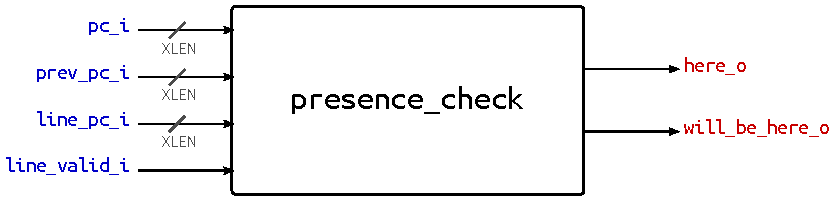
\includegraphics{img/presence_check-top.pdf}
  \caption{Presence checker module ports}
  \label{fig:presence_check-top}
\end{figure}
\begin{figure}[hbt]
  \centering
  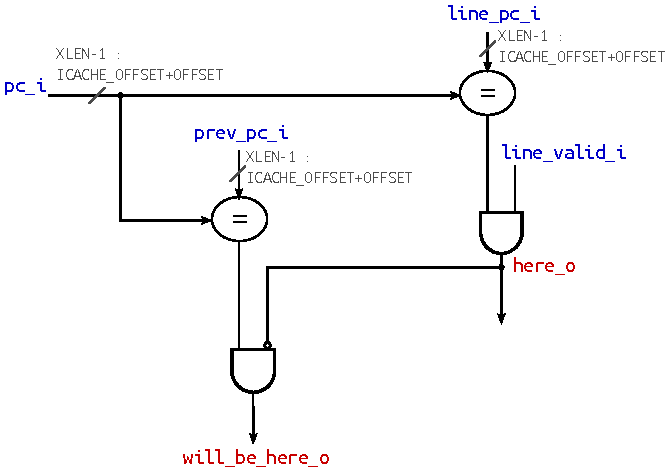
\includegraphics{img/presence_check.pdf}
  \caption{Presence checker combinational network}
  \label{fig:presence_check}
\end{figure}
The instruction selector block (see \cref{fig:presence_check-top,fig:presence_check}) features a simple combinational network that performs two checks in parallel to determine the need of a new cache access by the \ac{IFU}, in particular:
\begin{itemize}
  \item If the current address refers to an instruction present in the line register and the saved line is valid, then the \texttt{here} signal indicates that no new cache read is needed and that the instruction is to be selected inside the line register.
  \item If the current address refers to an instruction in the same cache line as the previous address, then either that line is already present in the line register, or it will be the next line read from the cache and so it will be saved as soon as the read completes. In this case a \texttt{will\_be\_here} signal tells the \ac{IFU} not to request the same line twice to the memory. 
\end{itemize}
If none of these signals are asserted, then a new cache request is sent to the interface.

All the instructions belonging to the same cache line have the same most significant parts of the addresses, namely only the $N$ \acsp{LSB} differ, where:
\begin{equation*}
  N = \lceil \log_2(\text{Instructions/cache line}) \rceil + 
      \lceil \log_2(\text{Bytes/instruction}) \rceil
\end{equation*}
So, to check whether two instructions belong to the same line, a comparison between the $64-N$ (or more generally $\texttt{XLEN}-N$, where \texttt{XLEN} is the parallelism of the processor) most significant bits of their addresses is sufficient. That is what the presence checker does as shown in \cref{fig:presence_check}.

\subsection{Instruction selector}
\begin{figure}[hbt]
  \centering
  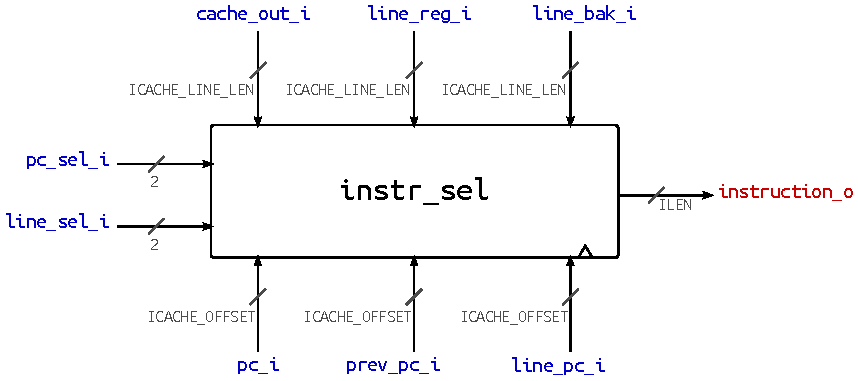
\includegraphics{img/instr_sel-top.pdf}
  \caption{Instruction selector module ports}
  \label{fig:instr_sel-top}
\end{figure}
\begin{figure}[hbt]
  %\hspace*{-1.5cm}
  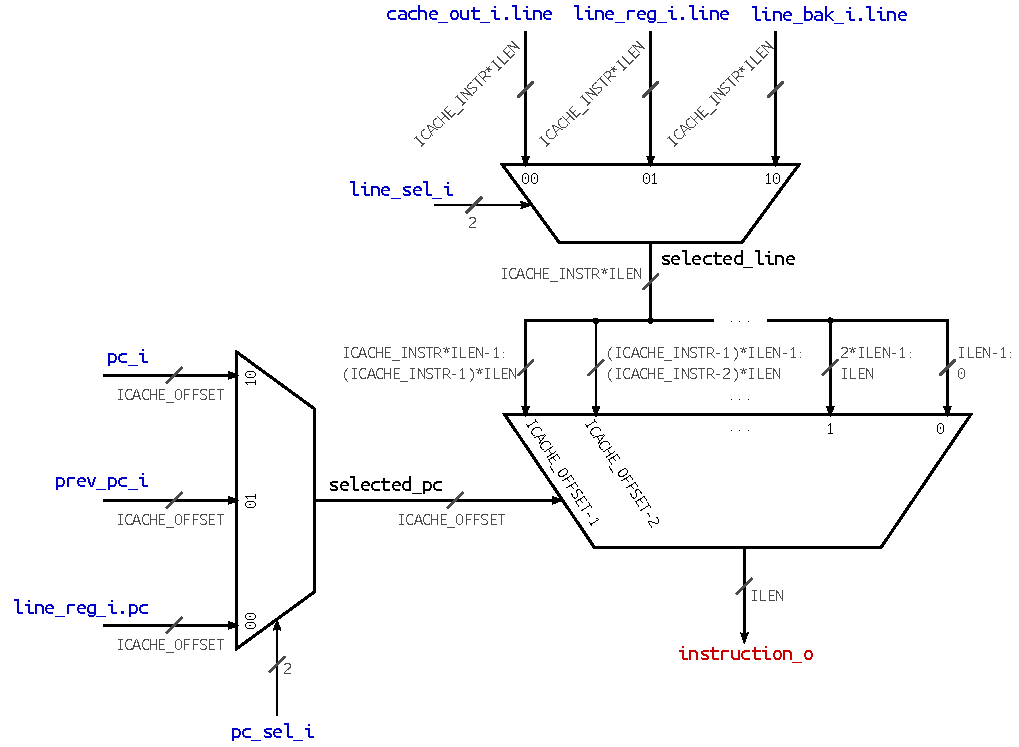
\includegraphics[width=\textwidth]{img/instr_sel.pdf}
  \caption{Selection network}
  \label{fig:instr_sel}
\end{figure}
The instruction selector takes as input all the three sources an instruction can be fetched from, three program counter sources\footnote{The only actually used source, as stated above, is the previous \ac{PC}, but the others were included in the initial version of the design and are kept for should a future need arise. Given that the synthesizer can optimize unused wires, this choice incurs in no overhead.} and the respective selection signals (see \cref{fig:instr_sel-top}). It outputs a single selected instruction to be pushed to the issue queue.

\Cref{fig:instr_sel} shows the combinational selection network of the instruction selector, which basically consists of two multiplexers selecting the desired cache line and the address pointing to that line and another multiplexer choosing the selected instruction inside such line.

According to the number of instructions stored in a single cache line, the output multiplexed can become quite large, nonetheless it should not be an issue in terms of total area.

\subsection{Fetch controller}

\section{\acf{BPU}}

\section{Branch unit}